\newpage
\section{Đề bài}

Dựa vào lý thuyết “Chapter 5 – Forecasting model of time series” đã học. Mỗi sinh viên hãy phân tích và thực hiện các yêu cầu bên dưới.

\textbf{Yêu cầu:}

\textbf{Phần A: Dùng công cụ Python, R và SPSS phân tích.}

\begin{enumerate}
    \item[] Dựa vào trang web Yahoo Finance (Figure \ref{fig:Yahoo}) bên dưới, hãy thực hiện các bước như sau:
    
    \begin{figure}[!htp]
    \centering
    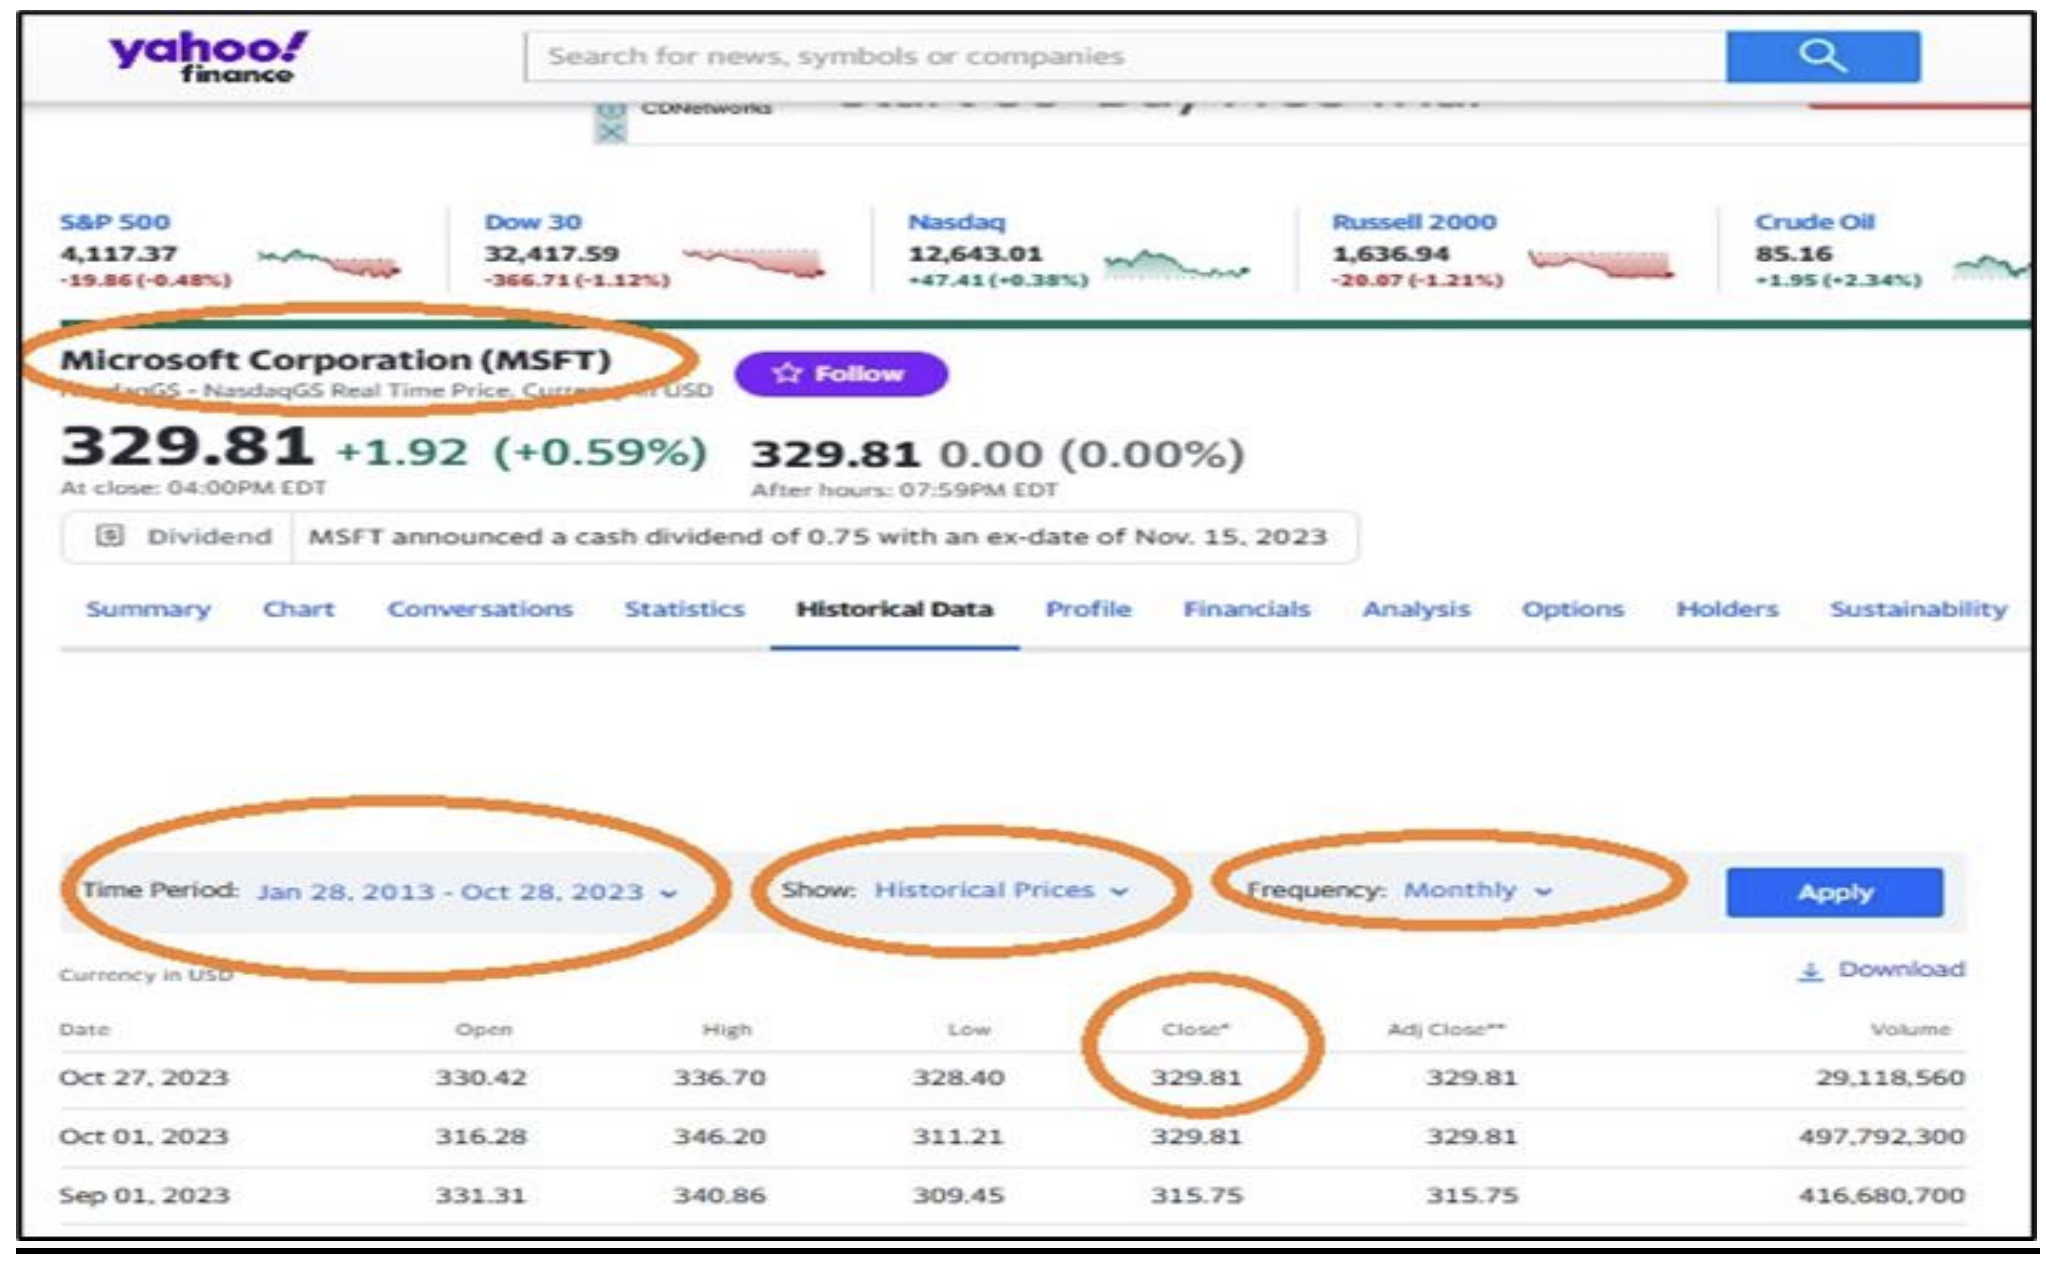
\includegraphics[width=0.95\textwidth]{LAB05/pics/YahooPage.png}
    \caption{Kết quả ước lượng tham số}
    \label{fig:Yahoo}
\end{figure}
    
    \item \textbf{Step 1.} Thu thập dữ liệu về giá đóng cửa (Close Price – sinh viên có thể tùy chọn dữ liệu theo ngày, tuần, hoặc tháng) của cổ phiếu MSFT (Microsoft Corporation) từ tháng giêng năm 2013 đến hiện nay tại trang web Yahoo Finance.
    
    \item \textbf{Step 2.} Plot biểu đồ giá đóng cửa và nhận xét dữ liệu có tính dừng hay không? Có hiện tượng gì? (xu hướng, vụ mùa, v.v.)
    \begin{itemize}
        \item Nếu dữ liệu có tính vụ mùa, sử dụng mô hình SARIMA thay vì mô hình ARIMA.
    \end{itemize}
    
    \item \textbf{Step 3.} Ước lượng dữ liệu dừng hoặc chưa dừng, dùng kiểm định ADF (Augmented Dickey Fuller).
    \begin{itemize}
        \item Nếu dữ liệu chưa dừng, tiến hành lấy sai phân “d” (bậc 1, bậc 2, v.v.).
        \item Kiểm tra lại tính dừng trên biểu đồ và kiểm định ADF sau khi lấy sai phân.
    \end{itemize}
    
    \item \textbf{Step 4.} Xác định AR(p) và MA(q)
    \begin{itemize}
        \item Plot ACF và PACF xác định “p” và “q”.
    \end{itemize}
    
    \item \textbf{Step 5.} Dự báo mô hình với p, d, và q.
    \begin{itemize}
        \item Tạo tập train, test (hoặc train, test, validate).
        \item Xây dựng và dự báo mô hình.
        \item Plot mô hình.
    \end{itemize}
    
    \item \textbf{Step 6.} Xác định các chỉ số MAE, RMSE, MSE, và MAPE.
    
    \item \textbf{Step 7.} Kết luận và đánh giá phân tích.
    
    \item \textbf{Step 8.} Xác định mô hình tốt nhất ARIMA (p, d, q) bằng auto arima (chọn lựa qua tiêu chí về chỉ số AIC và BIC) và so sánh với kết quả tại Step 3 và 4.
\end{enumerate}

\textbf{Chú ý:}

\begin{itemize}
    \renewcommand{\labelitemi}{-}
    
    \item Kết quả phần (A) phải được tóm tắt và chụp hình đưa vào tệp tin có quy cách đặt tên như sau: 
    \texttt{MSSV\_Họtên\_Lab05\_Output.docx (.pdf)}
    
    \item Gửi đính kèm các file SPSS, R, Python và dataset của Phần A. Tương tự, quy cách đặt tên file như sau:
    \begin{itemize}
        \renewcommand{\labelitemii}{$+$}
        \item \texttt{MSSV\_Họtên\_Lab05\_SPSS.sav (và .spv)}
        \item \texttt{MSSV\_Họtên\_Lab05\_Python.ipynb}
        \item \texttt{MSSV\_Họtên\_Lab05\_R.r}
        \item \texttt{MSSV\_Họtên\_Lab05\_Dataset.xlsx (.sav)}
    \end{itemize}
    \item (Ghi chú: nếu dataset file lớn, có thể lưu trên cloud và share đường link).
    
    \item Đóng gói lại thành 01 tập tin duy nhất và nộp file này theo đúng deadline với quy cách đặt tên file như sau: 
    \texttt{MSSV\_Họtên\_Lab05.rar (.zip)}
    
    \item Deadline nộp bài: 08/04/2026.
    
    \item Sinh viên nộp bài Lab05 không đúng deadline, xem như không có bài Lab05.
    
    \item Sinh viên nộp không đủ file và đặt tên không đúng quy cách tên file, sẽ bị trừ điểm.
    
    \item Các bài có hình thức trình bày và nội dung giống nhau sẽ nhận điểm Zero.
    
\end{itemize}